\newcommand{\cov}{\text{cov}}

\newcommand{\0}{\mathbf{0}}

\newcommand{\C}{\mathbf{C}}
%\newcommand{\A}{\mathbf{A}}
\newcommand{\X}{\mathbf{X}}
\newcommand{\U}{\mathbf{U}}
\renewcommand{\V}{\mathbf{V}}
\newcommand{\M}{\mathbf{M}}
\newcommand{\Q}{\mathbf{Q}}
\renewcommand{\H}{\mathbf{H}}
\newcommand{\I}{\mathbf{I}}
%\newcommand{\K}{\mathbf{K}}
%\newcommand{\W}{\mathbf{W}}
\newcommand{\R}{\mathbf{R}}
%\newcommand{\N}{\mathbf{N}}
\renewcommand{\P}{\mathbf{P}}
\renewcommand{\L}{\mathbf{L}}

\renewcommand{\a}{\mathbf{a}}
\newcommand{\h}{\mathbf{h}}
\renewcommand{\r}{\mathbf{r}}
\newcommand{\x}{\mathbf{x}}
%\newcommand{\s}{\mathbf{s}}
\renewcommand{\k}{\mathbf{k}}
\newcommand{\y}{\mathbf{y}}
\newcommand{\z}{\mathbf{z}}

\newcommand{\SSigma}{\mathbf{\Sigma}}
\newcommand{\GGamma}{\mathbf{\Gamma}}

\newcommand{\ttheta}{\boldsymbol\theta}
\newcommand{\eeta}{\boldsymbol\eta}
\newcommand{\vvarepsilon}{\boldsymbol\varepsilon}
\newcommand{\xxi}{\boldsymbol\xi}
\newcommand{\mmu}{\boldsymbol\mu}

\section{Data}

\subsection{Chlorophyll data}

We use CCI monthly and 8-days CHL data.

\begin{quotation}

Satellite data provide chlorophyll (CHL) concentrations with a spatial and
temporal resolution not achievable with in situ observations, making them
particularly relevant to the Red Sea, where very few in situ data collection
are conducted.

Level-3 mapped data from the NASA \mbox{SeaWiFS} (Sea-Viewing Wide
Field-of-View Sensor) satellite sensor are used in this study. The dataset is
publicly available at \texttt{http://oceancolor.gsfc.nasa.gov}. In this study,
we use the 9km resolution mapped weekly averages from January 1998 to December
2007 (460 time steps). At each time step, a $133\times 188$ pixel map is
available for a domain extending from longitudes between $33^\circ$E and
$44^\circ$E and latitudes between $12^\circ$N and $28^\circ$N, of which 5635
pixels correspond to actual Red Sea surface (see Figure \ref{figure1}(a)). A
log-transformation was applied in order to obtain an approximately Gaussian
distribution \cite{Campbell1995}. Pixels with too few observations were
discarded, and a control quality check was applied to remove outliers
\cite{Willis2004}.

Remotely sensed CHL may have missing data because of cloud coverage. The cloud
variability in the Red Sea follows a seasonal cycle. Figure \ref{figure1}(c)
shows that the cloud coverage is particularly pronounced during summers because
of the monsoon and it is sparse during winters. The cloud coverage is, however,
not homogenous over the Red Sea. It is much more pronounced in the south
(figure \ref{figure1}(b)). In this region, almost no data are available during
summers.

%\begin{figure}[h] \centering \includegraphics{../png/figure1.png} \caption{Raw
%data plots: (a) map of average log-concentrations of CHL between 1998 and 2004,
%(b) map of average percentage of missing data for each location between 1998
%and 2006, and (c) time-series of the percentage of missing data over the Red
%Sea between 1998 and 2004.} \label{figure1} \end{figure}


\end{quotation}

\subsection{DINEOF}

CCI data present missing data, in particular, in the southern Red Sea during
summer. In order to have a complete dataset on which can apply a clustering
algorithm, we use DINEOF, a data filling algorithm. The Chl data is averaged
over each region to give a data time-series for each of them.

\begin{quotation} The DINEOF (Data Interpolating Empirical Orthogonal Function)
is an EOF-based, recursive method for the reconstruction of data matrices with
missing values \cite{Beckers2003, Alvera-Azcarate2009}. It estimates the values
of the missing data by successive singular values decompositions (SVD) of a
given data matrix and truncated reconstructions. The advantage of this method
is that it does not require any a priori information about the data. It has
been successfully used for reconstruction of incomplete chlorophyll datasets in
different regions of the ocean \cite{Miles2010,Sirjacobs2011,Waite2013}.

Let $\X$ be an $m \times k$ centered data matrix with missing values initially
filled with 0s.  Then, until the missing values have converged, the following
steps are repeated. An SVD is first applied to the data matrix: $\X = \U\SSigma
\V^T$, with $\U$ an $m\times m$ unitary matrix, $\SSigma$ an $m\times k$
diagonal matrix and $\V$ a $k\times k$ unitary matrix. The missing values are
then replaced by the truncated reconstruction order $n$ of the data matrix:
$\{\X\}_{i,j} = \{\U^{(n)}\SSigma^{(n)} (\V^{(n)})^T)\}_{i,j}$, for $i,j$
indices of the missing values, with $\U^{(n)}$ the $m\times n$ matrix composed
of the $n$ first columns of $\U$, $\V^{(n)}$ the $k\times n$ matrix composed of
the $n$ first columns of $\V$, and $\SSigma^{(n)}$ the $n\times n$ diagonal
matrix with the $n$ largest eigenvalues on its diagonal. It is assumed that the
eigenvalues and eigenvector are sorted by decreasing order of eigenvalues. In
\cite{Alvera-Azcarate2009}, the authors introduced the filtering of the
temporal covariance matrix as a way of reducing spurious oscillations that may
appear when the data are sparsely sampled in time. This filtering is controlled
by the parameter of the Laplacian filter and the number of times the filter is
applied.

The values of the DINEOF parameters are determined following the method
outlined in \cite{Alvera-Azcarate2009}. The smoothing parameter of the
Laplacian filter is set to 0.005. The number of modes in the truncation and the
number of times the filter is applied are chosen following a cross-validation
technique. A random subset of observed values is taken from $X$ and assumed to
be missing before the DINEOF is applied. The algorithm is then run with
different numbers of iterations (1, 3, 10, 30, 100) and orders of truncation
(from 2 to 50). The set of parameters minimizing the RMS error over the
cross-validation data is chosen as the best number of iterations and order of
truncation. The approach of \cite{Beckers2006} is followed to select a
cross-validation dataset. Instead of selecting it by sampling the dataset point
by point, contiguous regions are set aside. These regions correspond to regions
of missing data from the original dataset and are selected randomly until 3\%
of the data have been extracted.

\end{quotation}

\subsection{Clustering}

We use clustering algorithm to divide the Red Sea into regions with similar
behavior. We tried K-means and Gaussian Mixture Model, a generalization of the
former.GMM was found to give better results.

\begin{quotation} I used clustering algorithms in order to derive the Red Sea
eco-regions. These were applied to monthly log-concentration of chlorophyll. I
used SeaWiFS data, that has been filled using DINEOF. I used the popular
K-means, and the Gaussian Mixture Model (GMM) clustering algorithms.

I found that GMM provides more robust results. With any number of clusters, we
obtain a division of the Red Sea into regions of comparable sizes.  With 5
clusters, the regions (shown in figure \ref{cluster}) are very similar to those
identified by \citet{Raitsos2013}.  Contrary to the purely latitudinal division
proposed by the former, we observe that the separation between clusters is
curved at the position of major Red Sea eddies.  The fact that the curvature is
oriented toward the south suggests that most nutrients propagate northward from
the Gulf of Aden.

%\begin{figure}[h] \centering
%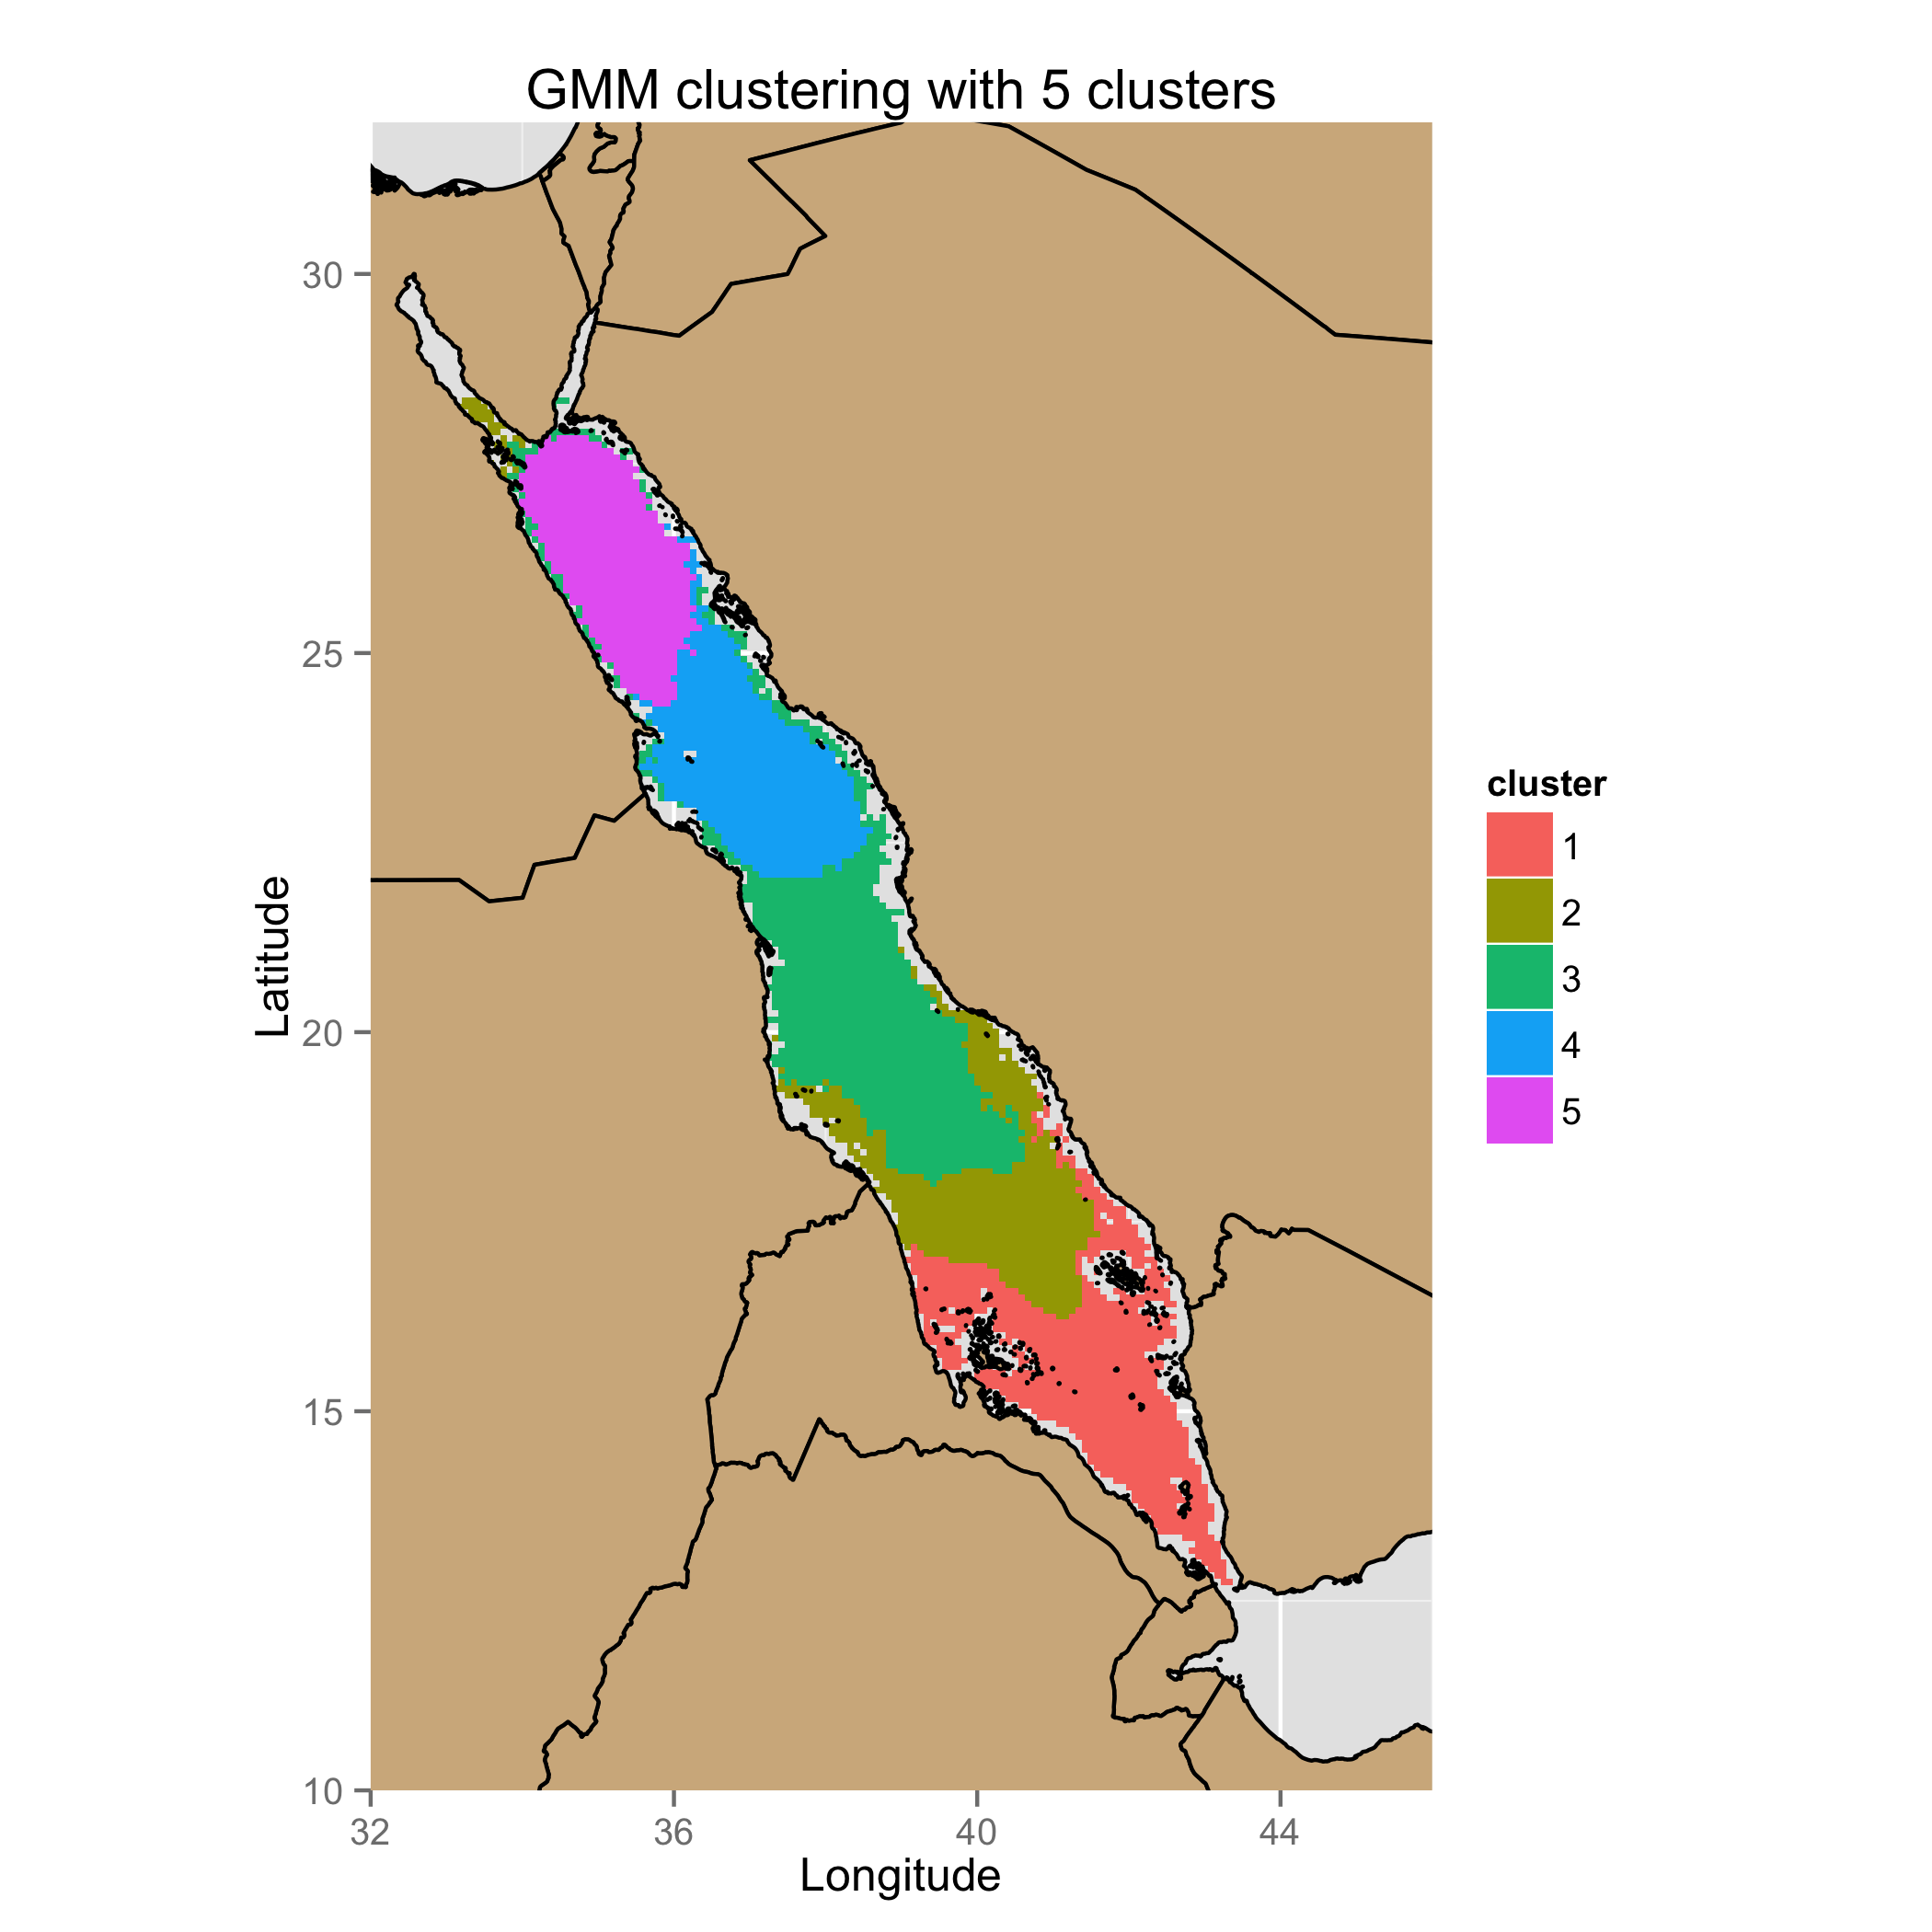
\includegraphics[scale=.15]{figures/clusters_k5.png} \caption{Clustering of Red
%Sea using GMM, with filled monthly SeaWiFS chlorophyll data.} \label{cluster}
%\end{figure}

In Chapter 2, I plan to use the dataset constructed in Chapter 1.  By using CCI
chlorophyll data instead of SeaWiFS, the need for data filling is minimized.
This is desirable, as data filling can introduce biases. It will also be
possible to use additional variables. For example, we can expect the
temperature and the bathymetry to have a large impact on the Red Sea
phytoplankton biology. Sea level anomaly can be useful in that it indicates the
presence of mesoscale eddies. Finally, alternative clustering algorithms will
be tested.  \end{quotation}

